\documentclass{article}
\usepackage[margin=21mm]{geometry}
\usepackage{booktabs,graphicx}
\title{Ion pad and electron SiPM readout}
\author{NAUSICAA analysis}
\date{29 October 2026}
\begin{document}
\maketitle
Six Julia processes collected 8,000 events from each MC sample in 186.84~s. 
Each retained ion cloud was mapped to pads; pure-Xe and Xe--15\%~He electron
clouds were assigned to EL holes and reduced to detected photoelectrons (PE)
per SiPM and time bucket. Every input carrier was assigned to a grid cell.
\begin{center}\small
\begin{tabular}{llrrrr}
\toprule
Sample & Readout & Input/event & Signal/event & Signal/input & Buckets/event\\
\midrule
bb0nu & ions & 112,143 & 112,143 & 1.00 & 1,466 \\
bb0nu & pure Xe e$^{-}$ & 112,106 & 14,981,352 & 133.64 & 958 \\
bb0nu & Xe--He e$^{-}$ & 112,129 & 14,734,431 & 131.41 & 378 \\
electrons & ions & 112,143 & 112,143 & 1.00 & 1,690 \\
electrons & pure Xe e$^{-}$ & 112,114 & 14,982,529 & 133.64 & 1,152 \\
electrons & Xe--He e$^{-}$ & 112,132 & 14,734,764 & 131.41 & 458 \\
\bottomrule
\end{tabular}\end{center}
\begin{center}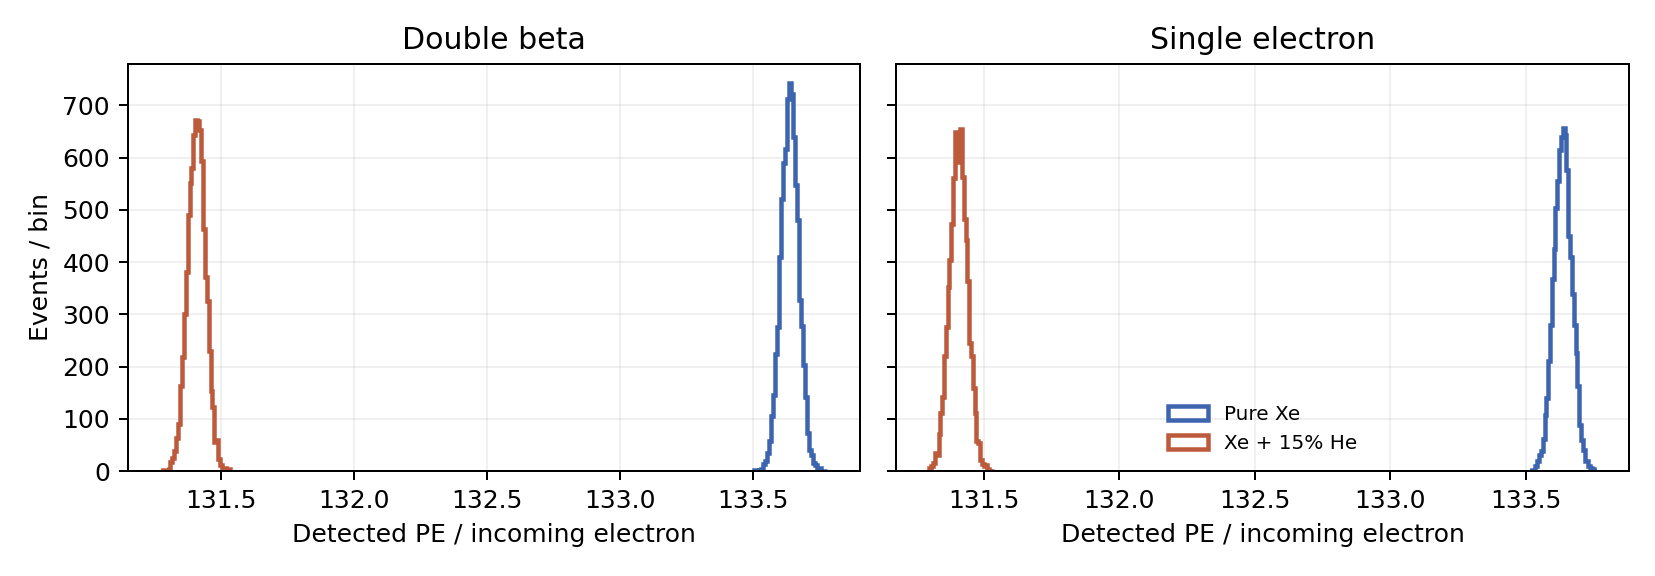
\includegraphics[width=.94\linewidth]{pe_per_electron.png}\end{center}
\paragraph{Grid and timing inputs.}
Ion pads have 2~mm pitch and 20~ms buckets at 0.1~m/s drift speed.
Electron holes have 10~mm pitch and 5~mm diameter, with 5~mm EL depth. PE are assigned to 2~microsecond buckets
at the configured conversion of 1~mm/microsecond. The ion and electron
arrival orders are opposite. An independent uniform phase is used for each
physical grid; the electron phase is shared by the two gas models of an event.
The EL reduced field is 3~kV/cm/bar at 15~bar, with gate/anode potentials 0/22500~V in a relative voltage gauge.
\paragraph{Optical model.}
The fitted mean EL yields from the Xe--He study are 2332.4 and 2293.5 photons per electron
for pure Xe and Xe--15\%~He. Photons are isotropic along the hole axis;
VUV rays touching the walls are absorbed. The analytic direct-light
acceptance is 0.190983 and the configured SiPM PDE is 30\%. The fitted yield is held at its mean;
PE counts are sampled with an exact binomial draw from the combined optical
acceptance and PDE. PE are placed in the parent electron's arrival bucket;
in-hole transit delay and electronics noise are outside this readout stage.
The Xe--He EL fits were measured near 1.2~bar; their use at 15~bar applies
reduced-field scaling.
\paragraph{Validation.}
The ion signal equals the retained input ion count in every event. Saved
grid indices and time buckets account for each signal; pure-Xe and Xe--He
readouts share a transverse grid phase per event. The complete event-wise
validation results accompany the HDF5 run summary.
\end{document}
